% test
% Template for PLoS
% Version 3.5 March 2018
%
% % % % % % % % % % % % % % % % % % % % % %
%
% -- IMPORTANT NOTE
%
% This template contains comments intended
% to minimize problems and delays during our production
% process. Please follow the template instructions
% whenever possible.
%
% % % % % % % % % % % % % % % % % % % % % % %
%
% Once your paper is accepted for publication,
% PLEASE REMOVE ALL TRACKED CHANGES in this file
% and leave only the final text of your manuscript.
% PLOS recommends the use of latexdiff to track changes during review, as this will help to maintain a clean tex file.
% Visit https://www.ctan.org/pkg/latexdiff?lang=en for info or contact us at latex@plos.org.
%
%
% There are no restrictions on package use within the LaTeX files except that
% no packages listed in the template may be deleted.
%
% Please do not include colors or graphics in the text.
%
% The manuscript LaTeX source should be contained within a single file (do not use \input, \externaldocument, or similar commands).
%
% % % % % % % % % % % % % % % % % % % % % % %
%
% -- FIGURES AND TABLES
%
% Please include tables/figure captions directly after the paragraph where they are first cited in the text.
%
% DO NOT INCLUDE GRAPHICS IN YOUR MANUSCRIPT
% - Figures should be uploaded separately from your manuscript file.
% - Figures generated using LaTeX should be extracted and removed from the PDF before submission.
% - Figures containing multiple panels/subfigures must be combined into one image file before submission.
% For figure citations, please use "Fig" instead of "Figure".
% See http://journals.plos.org/plosone/s/figures for PLOS figure guidelines.
%
% Tables should be cell-based and may not contain:
% - spacing/line breaks within cells to alter layout or alignment
% - do not nest tabular environments (no tabular environments within tabular environments)
% - no graphics or colored text (cell background color/shading OK)
% See http://journals.plos.org/plosone/s/tables for table guidelines.
%
% For tables that exceed the width of the text column, use the adjustwidth environment as illustrated in the example table in text below.
%
% % % % % % % % % % % % % % % % % % % % % % % %
%
% -- EQUATIONS, MATH SYMBOLS, SUBSCRIPTS, AND SUPERSCRIPTS
%
% IMPORTANT
% Below are a few tips to help format your equations and other special characters according to our specifications. For more tips to help reduce the possibility of formatting errors during conversion, please see our LaTeX guidelines at http://journals.plos.org/plosone/s/latex
%
% For inline equations, please be sure to include all portions of an equation in the math environment.  For example, x$^2$ is incorrect; this should be formatted as $x^2$ (or $\mathrm{x}^2$ if the romanized font is desired).
%
% Do not include text that is not math in the math environment. For example, CO2 should be written as CO\textsubscript{2} instead of CO$_2$.
%
% Please add line breaks to long display equations when possible in order to fit size of the column.
%
% For inline equations, please do not include punctuation (commas, etc) within the math environment unless this is part of the equation.
%
% When adding superscript or subscripts outside of brackets/braces, please group using {}.  For example, change "[U(D,E,\gamma)]^2" to "{[U(D,E,\gamma)]}^2".
%
% Do not use \cal for caligraphic font.  Instead, use \mathcal{}
%
% % % % % % % % % % % % % % % % % % % % % % % %
%
% Please contact latex@plos.org with any questions.
%
% % % % % % % % % % % % % % % % % % % % % % % %

\documentclass[10pt,letterpaper]{article}
\usepackage[top=0.85in,left=2.75in,footskip=0.75in]{geometry}

% amsmath and amssymb packages, useful for mathematical formulas and symbols
\usepackage{amsmath,amssymb}

% Use adjustwidth environment to exceed column width (see example table in text)
\usepackage{changepage}

% Use Unicode characters when possible
\usepackage[utf8x]{inputenc}

% textcomp package and marvosym package for additional characters
\usepackage{textcomp,marvosym}

% cite package, to clean up citations in the main text. Do not remove.
\usepackage{cite}

% Use nameref to cite supporting information files (see Supporting Information section for more info)
\usepackage{nameref,hyperref}

% line numbers
\usepackage[right]{lineno}

% ligatures disabled
\usepackage{microtype}
\DisableLigatures[f]{encoding = *, family = * }

% color can be used to apply background shading to table cells only
\usepackage[table]{xcolor}

% array package and thick rules for tables
\usepackage{array}

% create "+" rule type for thick vertical lines
\newcolumntype{+}{!{\vrule width 2pt}}

% create \thickcline for thick horizontal lines of variable length
\newlength\savedwidth
\newcommand\thickcline[1]{%
  \noalign{\global\savedwidth\arrayrulewidth\global\arrayrulewidth 2pt}%
  \cline{#1}%
  \noalign{\vskip\arrayrulewidth}%
  \noalign{\global\arrayrulewidth\savedwidth}%
}

% \thickhline command for thick horizontal lines that span the table
\newcommand\thickhline{\noalign{\global\savedwidth\arrayrulewidth\global\arrayrulewidth 2pt}%
\hline
\noalign{\global\arrayrulewidth\savedwidth}}


% Remove comment for double spacing
%\usepackage{setspace}
%\doublespacing

% Text layout
\raggedright
\setlength{\parindent}{0.5cm}
\textwidth 5.25in
\textheight 8.75in

% Bold the 'Figure #' in the caption and separate it from the title/caption with a period
% Captions will be left justified
\usepackage[aboveskip=1pt,labelfont=bf,labelsep=period,justification=raggedright,singlelinecheck=off]{caption}
\renewcommand{\figurename}{Fig}

% Use the PLoS provided BiBTeX style
\bibliographystyle{plos2015}

% Remove brackets from numbering in List of References
\makeatletter
\renewcommand{\@biblabel}[1]{\quad#1.}
\makeatother



% Header and Footer with logo
\usepackage{lastpage,fancyhdr,graphicx}
\usepackage{epstopdf}
%\pagestyle{myheadings}
\pagestyle{fancy}
\fancyhf{}
%\setlength{\headheight}{27.023pt}
%\lhead{\includegraphics[width=2.0in]{PLOS-submission.eps}}
\rfoot{\thepage/\pageref{LastPage}}
\renewcommand{\headrulewidth}{0pt}
\renewcommand{\footrule}{\hrule height 2pt \vspace{2mm}}
\fancyheadoffset[L]{2.25in}
\fancyfootoffset[L]{2.25in}
\lfoot{\today}

%% Include all macros below

\newcommand{\lorem}{{\bf LOREM}}
\newcommand{\ipsum}{{\bf IPSUM}}

%% END MACROS SECTION


\begin{document}
\vspace*{0.2in}

% Title must be 250 characters or less.
\begin{flushleft}
{\Large
\textbf\newline{Instantaneous Reproduction Number Estimation From Modelled Incidence}
}
\newline
% Insert author names, affiliations and corresponding author email (do not include titles, positions, or degrees).
\\
Robert Challen\textsuperscript{1,2*},
Leon Danon\textsuperscript{1,2}
\\
\bigskip
\textbf{1} AI4CI, University of Bristol, Bristol, UK.\\
\textbf{2} Department of Engineering Mathematics, University of Bristol, Bristol, UK.\\
\bigskip

% Insert additional author notes using the symbols described below. Insert symbol callouts after author names as necessary.
% Use the asterisk to denote corresponding authorship and provide email address in note below.
* rob.challen@bristol.ac.uk

\end{flushleft}
% Please keep the abstract below 300 words
\section*{Abstract}

TODO

% Please keep the Author Summary between 150 and 200 words
% Use first person. PLOS ONE authors please skip this step.
% Author Summary not valid for PLOS ONE submissions.

% \section*{Author summary}
%
% TODO \cite{ramanan2017}

\linenumbers

% Use "Eq" instead of "Equation" for equation citations.
\section*{Introduction}

Estimating the time varying reproduction number ($R_t$) is an important part of monitoring the progression of an epidemic, it informs short term projections of the epidemic size and hence guides decisions on policy interventions targetting behaviour \cite{gostic2020}. Changes in $R_t$ can reflect significant events in a pandemic such as the emergence of novel variants \cite{davies2021}. $R_t$ estimation may be done using a range of techniques with varying degrees of complexity \cite{abbott2024,alvarez2021,parag2021,thompson2019,wallinga2006,steyn2024,nash2023,nash2022,cauchemez2006,hong2020,johnson2021,ogi-gittins2024}, but the majority are based on a time series of count data reflecting the incidence of infection in the population. Such count data may be new infections, hospitalisations or deaths, and are well known to exhibit specific biases due to incomplete ascertainment, reporting delay, and right truncation, along with more generic data quality issues such as missing values or anomalous values \cite{abbott2020}.

When correcting for such issues, one approach is to use count data to estimate incidence of a disease ($I_t$) using a model based around a time varying Poisson rate ($\lambda_t$), and fitted using maximum likelihood, using a logarithmic link function. In this common situation the estimate of the Poisson rate at any given time point ($t$) is a log-normally distributed quantity defined by parameters $\mu_t$ and $\sigma_t$, which include a representation of the uncertainty in the data. It is appealing to use such a modelled incidence estimate as the basis for an estimate of $R_t$, and include this uncertainty into $R_t$ estimates. Incidence models can be derived in a number of ways, they are easily inspected for error and can be made tolerant of missing values and outliers.

A detailed review of the reproduction number is out of scope of this paper, and is well covered by Vegvari et al.\cite{vegvari2022}, who highlight the difference between instantaneous and case reproduction numbers. The case reproduction number is the average number of secondary cases that arise from individuals infected today, and can only be estimated once these secondary cases have occurred. The instantaneous reproduction number estimates the number of primary infections in the past that have resulted in the secondary infections observed today, and hence is used for real time pandemic monitoring \cite{gostic2020}. We concentrate solely on the instantaneous reproduction number in this paper. A key requirement for the estimation of the reproduction number is a profile of when secondary infections occur with respect to primary infections. This is described as the infectivity profile, a time dependent probability distribution, and is equivalent to the generation time distribution \cite{gostic2020,park2021}. The timing of sequential infections measured by the generation time is not directly observed, so the temporal distribution of the serial interval between the positive test results, or symptom onsets, of known infector-infectee pairs is often used as a proxy \cite{park2021, thompson2019}. The canonical framework for estimation of the instantaneous reproduction number direct from case data is the Cori method, as implemented in the R package `EpiEstim' \cite{thompson2019}.

This paper presents a mathematical approach to estimating the instantaneous reproduction number from modelled incidence data, given an estimate of the infectivity profile, and which propagates incidence model uncertainty into estimates of the reproduction number, which we from this point refer to as `$R_t$ from incidence'. We validate this method against a simulation based on a branching process model with fixed infectivity profile and parameterised reproduction number and compare the output to reproduction number estimates using the Cori method implemented in the R package `EpiEstim' \cite{thompson2019}.

Supporting implementations of all methods described here are provided in the associated R package ``ggoutbreak'' (\url{https://ai4ci.github.io/ggoutbreak/}).

\section*{Materials and methods}

\subsection*{Mathematical analysis}

To use a modelled estimate of incidence to predict $R_t$ we need to propagate uncertainty in incidence into our $R_t$ estimates. To calculate $R_t$ we can use the backwards-looking renewal equations \cite{gostic2020} which incorporate the infectivity profile of the disease ($\omega$) at a number of days after infection ($\tau$):

\begin{eqnarray}
\begin{aligned}
I_t &\sim Poisson(\lambda_t) \\
\lambda_t &\sim Lognormal(\mu_t,\sigma_t) \\
R_t &= \frac{I_t}{\sum_{\tau}{\omega_{\tau}I_{t-\tau}}}
\end{aligned}
\end{eqnarray}

giving us:

\begin{eqnarray}
\begin{aligned}
R_t &\sim \frac{\lambda_t}{\sum_{\tau}{\omega_{\tau}\lambda_{t-\tau}}} \\
R_t &\sim \frac{Lognormal(\mu_t,\sigma_t)}{\sum_{\tau}{
  Lognormal( \mu_{t-\tau} + log(\omega_{\tau}) , \sigma_{t-\tau})
}}
\end{aligned}
\end{eqnarray}


As an aside, it has been shown that the sum of log-normal distributions can be approximated by another log-normal \cite{lo2013} with parameters $\mu_Z$ and $\sigma_Z$.

\begin{eqnarray}
\begin{aligned}
	S_+ &= \operatorname{E}\left[\sum_i X_i \right] = \sum_i
	\operatorname{E}[X_i] \\
	&= \sum_i e^{\mu_i + \frac{1}{2}\sigma_i^2}
	\\
	\sigma^2_{Z} &= \frac{1}{S_+^2} \, \sum_{i,j}
	  \operatorname{cor}_{ij} \sigma_i \sigma_j \operatorname{E}[X_i] \operatorname{E}[X_j] \\
	  &= \frac{1}{S_+^2} \, \sum_{i,j}
	  \operatorname{cor}_{ij} \sigma_i \sigma_j e^{\mu_i+\frac{1}{2}\sigma_i^2}
	  e^{\mu_j+\frac{1}{2}\sigma_j^2}
	\\
	\mu_Z &= \ln\left( S_+ \right) - \frac{1}{2}\sigma_{Z}^2
\end{aligned}
\end{eqnarray}

The sum term in the denominator of the renewal equation consists of a set of correlated scaled log normal distributions with both scale and correlation defined by the infectivity profile ($\omega$). In our case $cor_{ij}$ can be equated to the infectivity profile ($\omega_{|i-j|}$) when $i \neq j$ and 1 when $i = j$. $\mu_i$ is $\mu_{t-\tau} + ln(\omega_{\tau})$.

\begin{eqnarray}
\begin{aligned}
	S_{t} &= \sum_{s=1}^{|\omega|} { \omega_s e^{\mu_{t-s} + \frac{1}{2}\sigma_{t-s}^2 }} \\
	\sigma_{Z,t} &= \sqrt{
	  \frac{
	    \sum_{i,j=1}^{|\omega|} {
  	    \big[\omega_{|i-j|}+I(i,j)\big] \omega_i \omega_j \big[\sigma_{(t-i)} e^{\mu_{(t-i)}+\frac{1}{2}\sigma_{(t-i)}^2}\big] \big[\sigma_{(t-j)} e^{\mu_{(t-j)}+\frac{1}{2}\sigma_{(t-j)}^2}\big]
	    }
	  }{S_{t}^2}
	}	\\
	\mu_{Z,t} &= \log\left( S_{t} \right) - \frac{1}{2}\sigma_{Z,t}^2
\end{aligned}
\end{eqnarray}

$\mu$ is the central estimate of case counts on the log scale, and its standard deviation $\sigma$ can be large. There are numerical stability issues dealing with terms involving $e^{(\mu+\sigma^2)}$, however keeping everything in log space and using optimised log-sum-exp functions this can be made computationally tractable \cite{blanchard2021}.

\begin{eqnarray}
\begin{aligned}
	\log(S_{t}) &= \log(\sum_{s=1}^{|\omega|} {  e^{\mu_{t-s} + \frac{1}{2}\sigma_{t-s}^2 + \log(\omega_s) }}) \\
	\log(T_{t,\tau}) &= \log(\omega_{\tau}) + \log(\sigma_{(t-{\tau})}) + \mu_{(t-{\tau})} + \frac{1}{2}\sigma_{(t-{\tau})}^2) \\
	\log(cor_{i,j}) &= \log(\omega_{|i-j|}+I(i=j)) \\
	\log(\sigma_{Z,t}^2) &= \log(
	    \sum_{i,j=1}^{|\omega|} {
  	      e^{
  	        \log(cor_{i,j}) + \log(T_{t,i}) + \log(T_{t,j})
  	      }
	    }) - 2 \log(S_{t}) \\
	\mu_{Z,t} &= \log( S_{t} ) - \frac{1}{2}\sigma_{Z,t}^2
\end{aligned}
\end{eqnarray}

N.B. if we assume the individual estimates of the incidence are uncorrelated this
simplifies to:

\begin{eqnarray}
\begin{aligned}
\log(\sigma_{Z,t}^2) &= \log(
	    \sum_{\tau=1}^{|\omega|} {
  	      e^{
  	        2 \log(T_{t,\tau})
  	      }
	    }) - 2 \log(S_{t})
\end{aligned}
\end{eqnarray}

% Empirically there is not a huge amount of difference in estimates between these
% two forms. If the infectivity profile $\omega$ is spread out over a large period
% then the correlation matrix will be $O(\omega)^2$ which may predicate this simpler
% order 1 formulation.

With $\mu_{Z,t}$ and $\sigma_{Z,t}$ we can derive a distributional form of $R_t$ incorporating uncertainty from modelled incidence estimates:

\begin{eqnarray}
\label{eq:final}
\begin{aligned}
R_t &\sim \frac{Lognormal(\mu_t,\sigma_t)}
{Lognormal( \mu_{Z,t}, \sigma_{Z,t})} \\
\mu_{R_t} &= \mu_t - \mu_{Z,t} \\
\sigma_{R_t} &= \sqrt{\sigma_t^2+\sigma_{z,t}^2} \\
R_t &\sim Lognormal(\mu_{R_t}, \sigma_{R_t})
\end{aligned}
\end{eqnarray}

This estimate of $R_t$ is conditioned on a single known infectivity profile. In reality there is also uncertainty in the infectivity profile ($\omega$) which plays a role in the definition of $\mu_{Z,t}$ and $\sigma_{Z,t}$. We cannot assume any particular distributional form for the infectivity profile, but we can use a range of empirical estimates of the infectivity profile to calculate multiple distributional estimates for $R_t$ and then combine these as a mixture distribution.

The nature of this mixture distribution will depend on the the various empirical infectivity profile distributions. However, we can use general properties of mixture distributions to create estimates for the mean and variance of the reproduction number estimate ($R_t^*$) combining the uncertainty arising from multiple infection profile estimates ($\Omega$) and from the incidence estimate model itself:

\begin{eqnarray}
\label{eq:final_2}
\begin{aligned}
E[R_t|\omega] &= e^{(\mu_{R_t,\omega} - \frac{1}{2}\sigma_{R_t,\omega}^2)} \\
V[R_t|\omega] &= \big[e^{(\sigma_{R_t,\omega}^2)} - 1\big] \big[e^{2 \mu_{R_t,\omega} + \sigma_{R_t,\omega}^2}\big] \\
E[R_t^*] &= \frac{1}{|\Omega|}\sum_{\omega \in \Omega} E[{R_t|\omega}] \\
V[R_t^*] &= \frac{1}{|\Omega|} \bigg[\sum_{\omega \in \Omega}{V[R_t|\omega]+E[R_t|\omega]^2}\bigg] - E[R_t^*]^2 \\
\end{aligned}
\end{eqnarray}

The cumulative distribution function of the mixture is simply the arithmetic mean of the component cumulative distribution functions (conditioned on each infectivity profile). If $\Phi$ is the cumulative distribution function of the standard normal distribution:

\begin{eqnarray}
\label{eq:final_3}
\begin{aligned}
F_{R_t^*}(x) &= \frac{1}{|\Omega|}\sum_{\omega \in \Omega}F_{R_t}(x|\omega) \\
P(R_t^* \le x) &= \frac{1}{|\Omega|}\sum_{\omega \in \Omega} P(R_{t,\omega} \le x) \\
P(R_t^* \le x) &= \frac{1}{|\Omega|}\sum_{\omega \in \Omega} \Phi\bigg(\frac{ln(x) - \mu_{R_t,\omega}}{\sigma_{R_t,\omega}}\bigg)
\end{aligned}
\end{eqnarray}

As the cumulative density function of this mixture distribution is a strictly increasing function, specific solutions for median ($q_{0.5}$) and 95\% confidence intervals ($q_{0.025}$ and $q_{0.975}$) can be calculated numerically by solving the following equations:

\begin{eqnarray}
\label{eq:final_4}
\begin{aligned}
\frac{1}{|\Omega|}\sum_{\omega \in \Omega} \Phi\bigg(\frac{ln(q_{0.025}) - \mu_{R_t,\omega}}{\sigma_{R_t,\omega}}\bigg) - 0.025 &= 0 \\
\frac{1}{|\Omega|}\sum_{\omega \in \Omega} \Phi\bigg(\frac{ln(q_{0.5}) - \mu_{R_t,\omega}}{\sigma_{R_t,\omega}}\bigg) - 0.5 &= 0 \\
\frac{1}{|\Omega|}\sum_{\omega \in \Omega} \Phi\bigg(\frac{ln(q_{0.975}) - \mu_{R_t,\omega}}{\sigma_{R_t,\omega}}\bigg) - 0.975 &= 0
\end{aligned}
\end{eqnarray}

Numerical solutions to this are moderately expensive to perform. A reasonable approximation can be expected by matching moments of a log normal distribution to the mean $E[R_t^*]$ and variance $V[R_t^*]$ of the mixture. This gives us the final closed form estimator for the reproduction number given a set of infectivity profiles, $\overline{R_{t,\Omega}}$, as:

\begin{eqnarray}
\begin{aligned}
\mu_{t|\Omega} &= log\bigg(\frac{E[R_t^*]^2}{\sqrt{E[R_t^*]^2 + V[R_t^*]}}\bigg) \\
\sigma_{t|\Omega} &= \sqrt{log\bigg(1 + \frac{V[R_t^*]}{E[R_t^*]^2}\bigg)}\\
\overline{R_{t|\Omega}} &\sim Lognormal(\mu_{t|\Omega},\sigma_{t|\Omega})
\end{aligned}
\end{eqnarray}

In summary we present a method for retrieving the distributional form of the reproduction number from estimates of incidence arising from simple statistical count models. This includes uncertainty arising from both count models and from infectivity profile distributions. It is fully deterministic and computationally inexpensive. It does not place any particular constraints on the nature of the infectivity profile distribution and can handle distributions that have a negative component, as is sometimes seen in serial interval estimates.

\subsection*{Validation}

To test this method we developed a simulation based on a branching process model parametrised by 5 different $R_t$ time series, a set number of imported infections at time zero, and fixed infectivity profile. Taken together, $R_t$ and the infectivity profile define the expected number of secondary infections given a primary infection, on each day post infection. This expectation is sampled using a Poisson distribution to realise simulated infections on each day. In each simulation run, the degree of outward edges in the network of realised infections at any given time is an instantaneous $R_t$. For each paramterisation of $R_t$ we generate 50 simulations with different random seeds, so that in bulk the simulation reproduction number will be close to the parameterised $R_t$. Each simulation generates a line list of synthetic infections. The line list of infected individuals were aggregated to daily counts of infection. Five random scenarios with different input $R_t$ time series parametrisation were considered, and 50 replicates of each scenario were simulated, with different random seeds, resulting in 250 simulations.

We are particularly interested in uncertainty propagation. To assess the effect of noise in the input case counts in subsequent $R_t$ estimates we assume that infection case counts are subject to varying degrees of ascertainment which change from day to day. The levels of ascertainment were applied to the same underlying infection time series, with observed counts being a binomial sample from the ``true'' infection counts for any given day. The probability of ascertainment on any given day was a random sample from a Beta distribution with a fixed mean, but three different coefficients of variation (parameter values in the supplementary materials). In this way there are three versions of each of the 250 simulations which have the same underlying infection counts, but whose case counts only vary by the degree of statistical noise in the observation of infections.

The resulting 750 observed infection counts were used directly as an input to `EpiEstim' to generate a set of baseline $R_t$ estimates, using a window of 14 days. The synthetic infection time-series were also used as input to estimate the underlying infection rate, using a simple statistical Poisson model with time varying rate parameter, represented by a piecewise polynomial of order 2, and fitted using maximum likelihood with a logarithmic link function according to the methods of Loader et al. \cite{loader1999} and a bandwidth equivalent to 14 days as implemented in the R package `locfit' \cite{loader2020}. The central estimate and the standard error of the fitted Poisson rate from this simple statical incidence model were used as inputs to the $R_t$ estimation method described in this paper, to derive an set of estimates of $R_t$ which are broadly equivalent to that produced by `EpiEstim'. This combined estimator is referred to as `$R_t$ from incidence'.

Both estimators were analysed for estimation delays, by identifying the minimum root mean squared error between estimate and true values when applied to a synthetic dataset designed for this purpose. The lags were corrected for by shifting the $R_t$ estimate by that appropriate number of days.

For each estimator method and within the 3 groups of low, medium and high ascertainment noise, 5 scenarios were run with 50 replicates of each scenario. The posterior distributions of daily $R_t$ estimates from both estimators, `EpiEstim' and `$R_t$ from incidence', were compared to simulation ground truth at all time points and summarised for each time series to give estimator performance metrics for each of the 750 simulation replicas. From the each of these replicas 20 bootstraps were resampled during summarisation (resulting in 15,000 sets of estimator metrics per method). Estimator metrics were graphically summarised to the 3 groups and presented as box-plots (main paper) and summarised to each of 5 scenarios within each of the 3 groups (supplementary). Comparisons between the two methods are made graphically.

We calculated the average continuous ranked probability score (CRPS) as a overall performance metric \cite{anderson1996,bosse2024,bosse2023,brocker2008,gneiting2007}. The average proportional bias of the estimates within each simulation, and the average universal residual gives us a measure of estimator bias. We calculated the mean of the 50\% interval width (inter-quartile range) of each estimate as a measure of estimator sharpness. We calculated the coverage probability of the 50\% inter quantile range as an indicator of estimator calibration. We further investigated calibration by de-biasing estimates and with these adjusted estimates derived a novel calibration metric as the Wasserstein distance \cite{panaretos2019} of the probability integral transform histogram from the uniform \cite{david1948,hamill2001,wilks2019,brockwell2007}. These metrics are more fully described in the supplementary materials.

We conducted two sensitivity analyses, one with an `EpiEstim' window and `locfit' bandwidth equivalent to 7 days, rather than the 14 in the main analysis, and a second comparing estimate quality when the estimates were not corrected for delays.

% As a final part of the validation we took the simulated individuals and applied a probability that the individual experienced symptoms, accoring to a Bernouilli distribution. For those who experienced symptoms, we applied a time delay representing a time from infection to onset of symptoms, defined by a Gamma distribution. From the first 1000 infector-infectee pairs who both experienced symptoms we calculated a serial interval, which we used to estimate an empirical serial interval distribution. We then counted the symptomatic individuals for each day of symptom onset, to get a daily symptomatic case count. From symptomatic case counts we use the same Poisson model with time varying rate as above, to derive a model of incidence of symptomatic cases rather than infections. We then test the methods described in this paper with symptomatic case counts and serial interval distribution to derive an estimate of $R_t$, which we compared to the parametrised input to the simulation, using CRPS and quantile bias as before.

% $$
% \begin{align}
% \frac{1}{|\Omega|}\sum_{\omega \in \Omega} \Phi\bigg(\frac{ln(R_{t,sim}) - \mu_{R_t,\omega}}{\sigma_{R_t,\omega}}\bigg)
% \end{align}
% $$

% Results and Discussion can be combined.
\section*{Results}

In Fig~\ref{fig1} panel A case counts and a modelled incidence estimate from a single simulation are shown for the 3 levels of ascertainment noise. Uncertainty in modelled incidence estimates increases with noise. In panel B we compare the $R_t$ estimates derived from this this simulation. `EpiEstim' can be observed to produce a slightly lagged estimate (top row panel B). In general the confidence of `EpiEstim' estimates appear related to the distance of the estimate from 1. The central estimate becomes more volatile with more noise in the data set, but the confidence intervals do not appear to change, suggesting noise in the input data does not affect uncertainty. Comparing to this `$R_t$ from incidence' (lower row panel B) is subject to less lag, and overall more uncertain, but otherwise agrees well with the `EpiEstim' estimate. Increased noise in the data increases the uncertainty of the Poisson rate estimates (panel A) and hence `$R_t$ from incidence' estimates, unlike `EpiEstim'.

% Place figure captions after the first paragraph in which they are cited.
\begin{figure}[!ht]
\centerline{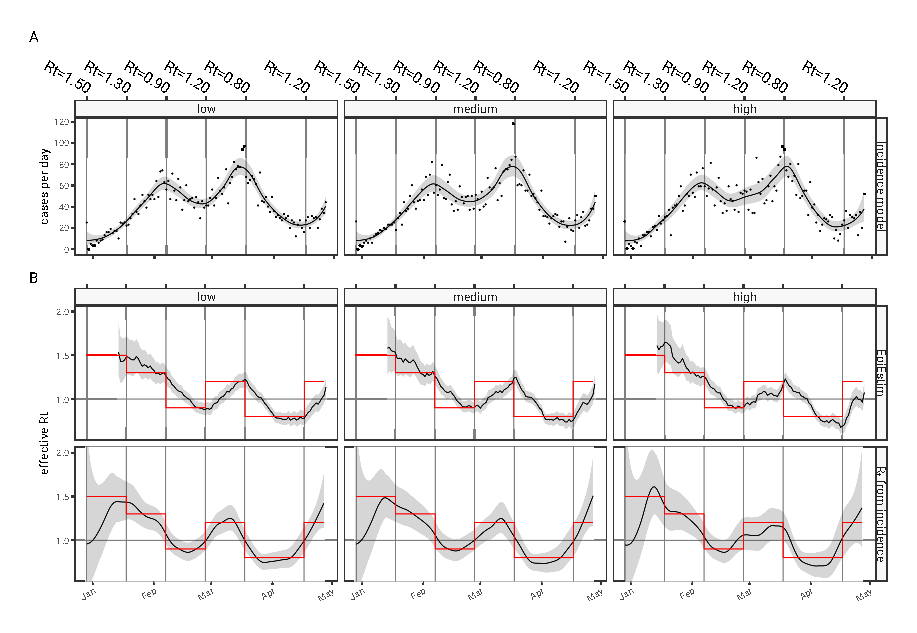
\includegraphics{fig/fig1-noise-qualitative}}
\caption{{\bf Instantaneous reproduction number estimates from a branching process model simulation.}
A qualitative comparison of instantaneous reproduction number estimates is shown. Panel A shows three case time series based on a single run of a branching process model parametrised with a stepped reproduction number time series (red lines in panel B) and infectivity profile as in supplementary figure 1. Case counts are shown as dots. A smoothed estimate of the cases per day as a line with shaded 95\% confidence intervals, based on a simple Poisson regression model. All three time series have on average 70\% case ascertainment, however the day to day variability of ascertainment is parameterised as a Beta distributed random variable, with ``low'', ``medium'' and ``high'' relating to the coefficient of variation of the Beta distribution (see supplementary materials). Panel B shows estimates of the reproduction number based on the methods presented in this paper, and in the top row `EpiEstim` estimates derived from the data points in panel A are shown. In the bottom row, $R_t$ estimates derived from the incidence model in Panel A using the methods described in this paper are shown. In panel B the parameterised $R_t$ is shown as a solid red line and can be regarded as the ground truth for this single simulation run.}
\label{fig1}
\end{figure}

In the main validation scenario we used a window for `EpiEstim' and `locfit' of 14 days. We saw in Fig~\ref{fig1} that this results in the estimate of $R_t$ lagging the true value. This is quantified in Tab~ref{tab1} and Fig~S1 in the supplementary materials. In the main analysis `EpiEstim' tends to produce an estimate delayed by 7 days and this lag is corrected by shifting the estimate in time before other metrics are calculated. In the first sensitivity analyses with a window of 7 days, a 4 day lag is observed for `EpiEstim', and in the second sensitivity analysis the metrics are calculated without correcting for lags.

\begin{table}[!ht]
\caption{{\bf Estimator delays in the validation scenarios}}
\centerline{\includegraphics{fig/tab1-lags}}
\label{tab1}
\end{table}

A quantification of the quality of the two estimation methods is shown in Fig~\ref{fig2} summarised from all 750 simulations, and corrected for estimator delays. In panel A the continuous ranked probability score is lower (better) for `$R_t$ from incidence' in all scenarios. In panel B the proportional difference between the true value and the median of the estimate probability (expressed as a percentage change) shows that the median of `EpiEstim` tends to slightly overestimate the true $R_t$ whereas `$R_t$ from incidence' exhibits little bias. This pattern is also seen in the average universal residual in panel C. In Fig~\ref{fig2} panel D, the 50\% prediction interval width is smaller for `EpiEstim' demonstrating a sharper, more confident, estimate than `$R_t$ from incidence', which has evidence of appropriately decreasing sharpness with increasing data noise. `EpiEstim' does not exhibit this deterioration in sharpness with noise. The low values of the probability of 50\% prediction coverage, as seen in panel E, which should be 0.5, implies that `EpiEstim` is over-confident in its predictions. Finally the PIT Wasserstein metric in Fig~\ref{fig2} panel F, allows us to compare the calibration of the 2 methods, one of which is over confident and the other being marginally underconfident on the same scale and suggests `$R_t$ from incidence' is better calibrated than `EpiEstim'.

\begin{figure}[!ht]
\centerline{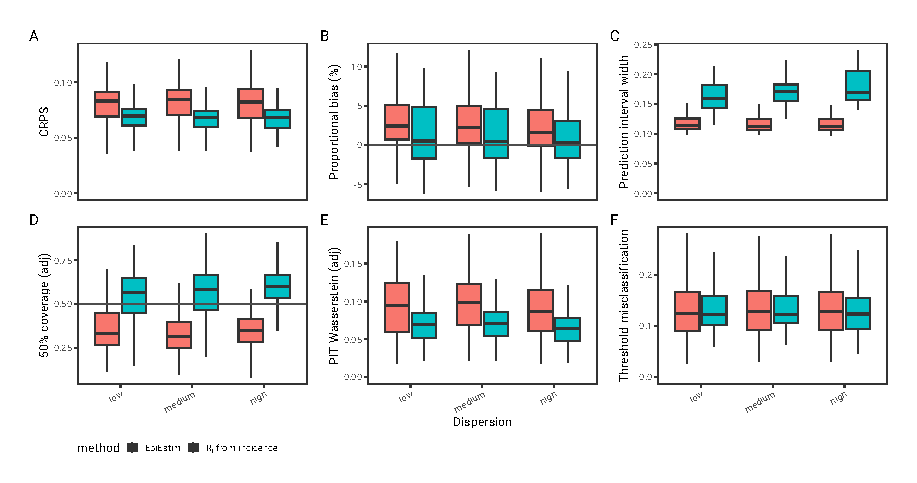
\includegraphics{fig/fig2-comparison}}
\caption{{\bf Quantitative comparison of $R_t$ estimation methods applied to 50 simulations of 5 scenarios at 3 levels of ascertainment noise.} The figure compares metrics describing the overall performance of the estimators with the continuous ranked probability score (CRPS) - lower is better, panel A; the average proportional bias, and mean universal residuals which characterise bias, in panel B and C - lower is better; The 50\% prediction interval width measures estimator sharpness and lower is better if the estimator is unbiased and well calibrated (panel D); and the probability of 50\% coverage (ideal value is 0.5, panel E), and adjusted probability integral transform (PIT) Wasserstein metric (lower is better, panel F)}
\label{fig2}
\end{figure}

In the first sensitivity analysis, the amount of data informing the $R_t$ estimates is reduced from 14 to 7 days, and produces very similar patterns to the main analysis except that, with less data to inform them `$R_t$ from incidence' estimates, they become excessively conservative in all but the high ascertainment noise scenarios (further details in the supplementary). In the second sensitivity analysis without correction for lag, `EpiEstim` estimates perform less well in all metrics as the lag penalises all dimensions of the quality of the estimator.

\section*{Discussion}

In this paper we describe a mathematical method for deriving an estimate of the effective reproduction number ($R_t$) from modelled estimates of disease incidence, that incorporates uncertainty from both incidence model and infectivity profile. We provide evidence that when combined with simple incidence models, our method produces $R_t$ estimates that are equivalent to, or an improvement on, the de-facto standard algorithm implemented in `EpiEstim' \cite{thompson2019}, when assessed against synthetic outbreak data. In contrast to `EpiEstim' our method produces estimates that reflect uncertainty in the data.

The method described here can be applied to any incidence model that produces time varying log-normally distributed incidence estimate. This includes a broad family of Poisson regression models \cite{nelder1972,loader1999,hastie2017}, or latent Gaussian models \cite{rue2009} using logarithmic link functions, and is agnostic to the formulation of those models. The incidence models can be estimated on time aggregated data \cite{nash2023}, include covariates such as day of week effects, or incorporate change points, without affecting the derivation of the reproduction number estimates. In terms of infectivity profile, our method is robust to distributions with zero or negative time intervals between index and secondary observations. It could therefore be used with directly observed real world serial interval distributions \cite{park2021} and delayed case counts as proxies for infectivity profile and infection incidence, which are necessarily inferred quantities; this is explored further in the `ggoutbreak' package documentation (\url{https://ai4ci.github.io/ggoutbreak/}). However, our method does not specifically address important questions arising from ascertainment bias, or right truncation of observed incidence, both of which would have to be addressed in the pre-requisite incidence models \cite{abbott2020,abbott2024}.

The validation comparison here uses a simple statistical model of incidence, combined with our method to derive $R_t$ estimates, versus estimates produced direct from the data by `EpiEstim'. This shows that the simple incidence model, and our $R_t$ derivation, produces estimates that appear less lagged that `EpiEstim`, with slightly less bias, and which have a more appropriate degree of confidence given their accuracy. We have not formally tested the statistical significance of these because they are based on a very large number of observations, and eveny tiny differences will be statistically significant.

Our method is not a like for like replacement for `EpiEstim' as it requires an incidence model, rather than directly using data, and comparing the two algorithms is therefore looking at both the incidence model and the method for deriving $R_t$. This must be bourne in mind when interpreting the validation section of this paper. By picking a very simple statistical model for incidence, to which to apply our method for estimating $R_t$, we hope to demonstrate that the combination is not obviously inferior to `EpiEstim'. If we had used more sophisticated incidence model the overall $R_t$ estimate may have very different characteristics.

A further limitation in our validation is that we pragmatically chose to simulate using a set of 5 step functions for $R_t$ parametrisation, which we expect to be relatively challenging for both `EpiEstim' and the simple statistical models for incidence we used here. We could have picked any other function to use for validation, and it is clear that relative performance between the methods varies with scenario (see supplementary materials). A more realistic smooth $R_t$ paramterisation time series has been performed and both methods perform better in such scenarios, so we consider our simulations to be worst case. There are likely to be scenarios where `EpiEstim' performs better.

We have used a set of generic metrics relevant to probabilistic predictions to analyse the bias, sharpness and calibration of $R_t$ estimators and we report and adjust for lag using a cross-correlation analysis. As $R_t$ estimators are time-series based there are additional temporal aspects in the validation that might have been informative. Whilst these generic metrics are informative the main value of an $R_t$ estimate is to answer the question ``is the epidemic increasing?'' and a dedicated metric for $R_t$ comparison which describes how accurately, and with what confidence, the estimator predicts when the $R_t$ value is greater than 1, would have been useful. In some situations it may be preferable to have an over sharp, poorly calibrated estimate if it is better at predicting the growth phases of the epidemic. This is a subject for further work.

Not withstanding these limitations in validation, we argue our method for deriving $R_t$ from log-normally modelled incidence estimates, which are commonly output by amongst statistical modelling frameworks, is a useful adjunct to the range of tools available for monitoring an epidemic. It is relatively quick and deterministic, and is flexible enough to be combined with a wide range of temporal incidence modelling techniques, which could account for reporting delays or ascertainment bias, or extended to spatio-temporal incidence models.

\nolinenumbers

\bibliography{refs}

\section*{Funding}

RC and LD are funded by UK Research and Innovation AI programme of the Engineering and Physical Sciences Research Council (EPSRC grant EP/Y028392/1;  \url{https://gow.epsrc.ukri.org/NGBOViewGrant.aspx?GrantRef=EP/Y028392/1}). RC and LD are affiliated with the JUNIPER partnership funded by the Medical Research Council (MRC grant MR/X018598/1; \url{https://www.ukri.org/councils/mrc/}). The views expressed are those of the authors.

\section*{Competing interests}

The authors have no competing interests to declare.

\section*{Author contributions}

RC and LD generated the research questions. RC performed the mathematical analysis and simulations, and created the supporting software package. RC and LD provided validation of the methods. LD provided supervision of the research. RC developed the first draft of the manuscript. RC and LD contributed to the final editing of the manuscript and its revision for publication and had responsibility for the decision to publish.

\section*{Data and code availability}

All data and code used for running experiments, model fitting, and plotting is available on a GitHub repository at \url{https://ai4ci.github.io/ggoutbreak-paper/}. The methods described here are implemented in the form of an R package to support the estimation of epidemiological parameters and it is deployed on the A14CI r-universe (\url{https://ai4ci.r-universe.dev/ggoutbreak}). We have also used Zenodo to assign a DOI to the repository: doi:10.5281/zenodo.7691196.

\section*{Supporting information}

% Include only the SI item label in the paragraph heading. Use the \nameref{label} command to cite SI items in the text.

\paragraph*{S1 Appendix.}
\label{S1_Appendix}
{\bf Simulation for validating Rt estimates, additional results and sensitivity analyses} Methodological details of simulation set up for validating the performance of $R_t$ estimators presented in the main paper, additional figures and detailed results from the sensitivity analyses.

\paragraph*{S2 Appendix.}
\label{S2_Appendix}
{\bf Metrics for evaluating the quality of probabilistic estimators.} Methodological details of performance metrics used for validating the performance of $R_t$ estimators presented in the main paper.

\end{document}

